\graphicspath{{ch6_sam_da/}{Figures/}}
% \graphicspath{{Figures/}}

\chapter{SAM-DA: Decoder Adapter \\for Efficient Domain Adaptation}
\chaptermark{SAM-DA: Decoder Adapter}
\label{chapter:samda}

\sidechaptersummary{Adapter for large segmentation models, supervised segmentation performance improvement, applications to domain generalization}

\subsubsection{Synopsis}This chapter addresses the domain adaptation challenge for semantic segmentation in medical imaging. Despite the impressive performance of recent foundational segmentation models like SAM on natural images, they struggle with medical domain images. Beyond this, recent approaches that perform end-to-end fine-tuning of models are simply not computationally tractable. To address this, we propose a novel SAM adapter approach that minimizes the number of trainable parameters while achieving comparable performances to full fine-tuning. The proposed SAM adapter is strategically placed in the mask decoder, offering excellent and broad generalization capabilities and improved segmentation across both fully supervised and test-time domain adaptation tasks. Extensive validation on four datasets showcases the adapter's efficacy, outperforming existing methods while training less than 1\% of SAM's total parameters.

\subsubsection{Publication}This chapter is based on a publication\JGT{CITE}, and its contents have been modified slightly to be more consistent with the rest of the thesis. More specifically, \Cref{fig:neural_diagram} and \Cref{tab:dataset_details_samda} have been added to the main text from the supplementary material, \Cref{tab:encoder_ablation_trained,tab:encoder_ablation_generalization} were a single table in the original publication and have been separated into two.

\subsubsection{Author contributions}The work in this chapter was done in collaboration with the University Hospital Bern. The contributing authors were Moritz Schmid, Pablo Márquez Neila, Sebastian Wolf, Martin Zinkernagel, and Raphael Sznitman. My contribution was the development and implementation of the method; conception and evaluation of the experiments and, together with the co-authors, writing of the paper.

\section{Introduction} \label{sec:intro}
%\subsection{Linear surface features on Europa}
% introduce bands, rc, db, ul here?

Different forms of lineaments may evolve out of initial cracks in the icy surface of Jupiter’s moon Europa\sidecite{Figueredo2004, Bradak2023b, Greenberg1998, ProckterPatterson2009}. Therefore, all types of lineaments have the potential to link to subsurface liquid water, as evidence is found for Enceladus\sidecite{Hansen2006, Sladkova2021, Ingersoll2016}. This makes lineaments of high interest to Europa's potential as a habitable world\sidecite{Daubar2024}.

\plainwidefig{1}{regional_mosaics/Figures/basemap_excerpt.png}{Global map with regional maps (RegMaps) in shades of red and the region for the manually revised lineament map (red box). Top: Basemap from USGS~\cite{USGS2002}. Bottom: Global geologic map~\cite{Leonard2024}.}{fig:RegMaps_basemap}

The Solid State Imager (SSI) onboard NASA’s Galileo spacecraft mapped approximately 10\% of Europa’s surface at a regional resolution of 200-230 m/px. Two north-south covering image mosaic swaths acquired under similar illumination conditions portray parts of the leading and trailing hemispheres (in the following abbreviated as ``RegMaps'', see \Cref{fig:RegMaps_basemap}). Because of the north-south extent and leading/trailing locations, these image mosaics enable the study of regional geological processes across a range of latitudes and longitudes\sidecite{Figueredo2003, Sarid2004, Patterson2006, Collins2022}. However, they do not enable features to be linked globally. 
Unfortunately, the most complete existing geologic maps\sidecite{Figueredo2004} of the RegMaps are not available in a digitised version. Furthermore, the level of detail with respect to the mapped lineaments is insufficient for an extensive lineament analysis due to the scale of the map. The map we present in this work is at a larger scale and therefore reveals fine lineae in areas previously mapped as ``ridged plains''\sidecite{Greeley2000}.

\plainwidefig{1}{regional_mosaics/Figures/Features_examples_grid.png}{A selection of Europan surface type features.}{fig:features_exs}

The surface of Europa is characterised by tectonic features overlaid by a small number of impact craters and disrupted in some regions by chaos terrain. Regional and global mapping has identified three broad episodes of deformation\sidecite{Prockter1999, Figueredo2000, DoggettEuropaBook2009, Leonard2024}. The oldest identifiable tectonic unit, ridged plains (\Cref{fig:features_exs}.A), is widespread across the surface. Characterised by multidirectional, mostly high-albedo linear ridges, the ridged plains unit overlaid by all later structures such that it appears as background plains material\sidecite{Daubar2024, Leonard2024}. Next in the stratigraphic sequence are bands, linear or curvilinear dilational features that have formed by symmetrical spreading from a crack or double ridge with new subsurface material filling the gap\sidecite{Greeley2000, Tufts2000}, analogous to mid-ocean ridges on Earth\sidecite{Sullivan1998} (\Cref{fig:features_exs}.B). Band morphologies fall into two major types: relatively smooth material comprised of small hummocks, and more rugged subparallel ridges\sidecite{Prockter2002}, that may be related to the band’s opening rate\sidecite{Stempel2005}. The youngest episode of deformation is the result of ``chaos'' formation, in which the surface has been disrupted from below, resulting in the breakup of preexisting terrain into discontinuous blocks of icy material set into a darker, hummocky matrix (\Cref{fig:features_exs}.C)\sidecite{Greeley2000}. Microchaos consists of smaller, discontinuous subcircular patches of chaos\sidecite{Pappalardo1998, Spaun2002, Noviello2019}, whose relationship to the larger chaos regions is not yet understood\sidecite{Collins2009}. Chaos may result from upwelling diapirs of thermally or compositionally buoyant material intersecting the surface\sidecite{Greenberg1999, Sotin2002, Figueredo2002, Schmidt2011, Collins2009} and it has been proposed that a periodic thinning and thickening of the ice shell drives periodic formation of chaos and regional plains terrain on a timescale comparable with the inferred surface age of 20 to 200 Myrs\sidecite{Bierhaus2009, Hussmann2004}. The regional plains unit makes up for 53\% of the global coverage, which makes it the most common unit, followed by chaos terrain with 40\%\sidecite{Leonard2024}. 

One feature that has formed throughout Europa’s stratigraphic history is the double ridge, which is widespread across the surface\sidecite{Figueredo2000}. Consisting of a distinct V-shaped trough flanked on each side by a single ridge\sidecite{Head1999, Greeley2000} (\Cref{fig:features_exs}.D), double ridges are observed at a range of size scales and as linear or curvilinear features a few tens of meters to hemispherical in length, and some forms appear related to diurnal tides\sidecite{Hoppa1999a}. Multiple models have been proposed for their formation, however, none are able to fully match all the observations\sidecite{ProckterPatterson2009, Daubar2024}. Ridge complexes are less common and consist of several adjacent parallel or anastomosing sets of double ridges\sidecite{Greeley2000} (\Cref{fig:features_exs}.E). Their formation mechanisms remain obscure\sidecite{Kattenhorn2009}. The youngest tectonic features on Europa are troughs, which appear similar to the V-shaped troughs of double ridges but lack the flanking ridges\sidecite{Greeley2000} (\Cref{fig:features_exs}.F). These are not observed in older terrains, perhaps because they fade and are overlooked easily\sidecite{Greeley2000}, but it is likely that they have been exploited to form other types of tectonic features\sidecite{Kattenhorn2009}. 
 
Because so little is known about how Europa’s tectonic features relate to the stresses that form them, including diurnal, non-synchronous, and polar wander\sidecite{Kattenhorn2009, Sotin2009}, the extent to which the tectonic landforms penetrate the ice shell is not well understood. Knowledge of the pathways that these features create or exploit is critical to understanding how material moves through the ice shell, and whether liquid water, including the ocean, is accessed. 
% End of Louise's paragraph

A global geologic map\sidenote{Such as the one in~\cite{Leonard2024}, or \Cref{fig:RegMaps_basemap}}, provides the global context for current missions to Europa, namely JUICE and Europa Clipper. The Europa Imaging System (EIS) on NASA's Europa Clipper will deliver a global view of Europa at a resolution $\leq$100 m/px in the 2030's\sidecite{TurtleSSR}. This global dataset will be valuable for lineament cross-cutting analyses and can, for the first time, result in a relative dating of globally interlinked regions\sidecite{Daubar2024}. The relative ages can be compared with absolute age results from crater counting\sidecite{Daubar2024}. Already for this reason alone, a global lineament map is valuable. Furthermore, spatially varying lineament characteristics, for example a regionally varying width of lineaments or different categorical distributions can be used to interpret the geological evolution of Europa's surface.

However, at 100~m/px, lineaments in background ridged plains appear as a dense network, which makes a complete lineament mapping time-consuming. This is where deep learning algorithms can help. \sidecite{Haslebacher2024a} have shown that an automated mapping framework with human validation reduces the workload while still accurately mapping 30-50~\% of lineaments. They trained a regional convolutional neural network, or Mask R-CNN\sidecite{He2018} for lineament mapping in Galileo images showing Europa's surface. Although the time used for mapping can be reduced with LineaMapper v1.0, the tool is not optimised for the resolution and illumination conditions of the RegMaps and would benefit from a larger training dataset. 
To maximise scientific return and flexibility in planning with EIS, an early preparation based on existing imagery is needed to ensure that the evaluation and analysis of all images is optimal. For this, we aim to improve LineaMapper's ability to correctly detect and segment a higher number of lineaments and to provide more continuous segmentation masks.

\plainwidefig[t]{1}{regional_mosaics/Figures/2024_07_17_apply_LineaMapper_scheme_optimised-01.png}{Workflow for assembling LineaMapper's predictions. A moving window tiling algorithm ensures overlapping areas for stitching the predictions together, which are based on smaller tiles of a context image. The need for such an algorithm is especially high for lineaments, which oftentimes run over an area larger than the tile size.}{fig:graphic_Stitching_algo}

Here, we attempt to map all identifiable lineaments in the Galileo RegMaps for an analysis of the evolution of lineament characteristics throughout their formation. This includes lineaments in the ridged plains, which have not frequently been mapped previously, but if mapped, a stratigraphy of lineaments inside ridged plains is insightful\sidecite{Bradak2023}.
To achieve this, we use a new methodology: We use the automated mapping tool LineaMapper\sidecite{Haslebacher2024a} together with a dedicated stitching algorithm to guide the mapping of the RegMaps iteratively. With 2140 new lineaments from a revised part of the RegMaps\sidenote{See red box in \Cref{fig:RegMaps_basemap}}, we train and release LineaMapper v1.1 and v2.0, which are optimised for the RegMaps. Subsequently, the complete Galileo RegMaps are fed into LineaMapper v1.1 and v2.0 and automatically assembled into a continuous lineament map of the RegMaps\sidenote{See \Cref{sec:fullRegMaps}.}.

We extract the length, the width, the azimuth, and the fragmentations per kilometre (FPK), which we use as an estimation of a lineaments relative age. With these extracted characteristics, a number of questions have the potential to be answered, which we explore in this work: 

\begin{enumerate}
    \item Is there a difference in the number or area density of lineaments in the chaos vs. ridged plains region?
    \item Does the data suggest that the distribution of lineament width, length, number of fragmentations, and FPK, for each lineament category is equal within chaos and ridged plains?
    \item Do we find correlations between lineament characteristics, and do the fits vary for the chaos and ridged plains unit?
    \item Can LineaMapper identify different terrain types (chaos and ridged plains) by lineament density?
\end{enumerate}

\textfig[t]{1}{regional_mosaics/Figures/galilean_moons_2023_Marseille_LineaMapper_workflow_circle.pdf}{Iterative cycle for improving LineaMapper and generating a near-complete lineament map.}{fig:circle_workflow}

\section{Method}
\label{sec:method}
%% Main points:
%% - Preliminary: explain SAM very briefly and how the decoder works
%% - Explain the adapter
%% - How we attach the adapter to the decoder of SAM
%% - Initialization of the adapter
%% - Why we use it in the decoder: less parameters. The encoder should give a good representation already
%% - Image showing everything
We propose a simple, lightweight adapter for the Segment Anything Model (SAM)\sidecite{sam} that draws inspiration from adaptation techniques in the NLP literature. 

\plainwidefig[t]{1}{Figures/method.pdf}{Illustration of the proposed adaption for SAM Decoder in layer~$\ell$. In each layer, the adaption embeddings are fed along with the dense embeddings to the trainable zero-initialized attention module. Then, the resulting tokens are combined with the decoder embeddings with a trainable gating parameter and a linear MLP.}{fig:method_samda}

\subsection{Segment Anything Model.}
\label{sec:sam}
SAM consists of three primary components: an image encoder, a prompt encoder, and a mask decoder. The image encoder is a standard MAE pre-trained Vision Transformer (ViT)\sidecite{dosovitskiy2021an} that transforms the input image into an embedding space. The prompt encoder takes either sparse (points, boxes) or dense (masks) annotation formats and produces encoded prompts. Both the image embedding and the encoded prompts are fed to the mask decoder, which consists of a transformer block with a mask prediction head. The transformer block applies two layers of two-way cross-attention operations acting on the image and the prompt embeddings. The result of the transformer is upsampled with an MLP and then fed to a linear classifier, which predicts the final segmentation mask.

\subsection{SAM Decoder Adapter.}
\label{sec:adapter}

The LLaMA-Adapter\sidecite{llama_adapter} is an adaption method originally introduced to fine-tune pre-trained LLMs such as LLaMA\sidecite{llama}. In the context of language generation, this adapter introduces a set of learnable adaption prompts at the higher layers of the LLaMA transformer, and prepends them to the word tokens before the attention operations. 

Our approach brings the idea of prompt-based adaptation from NLP to SAM. We introduce a new learnable adaption prompt~$A_\ell\in\real^{N\times{}D}$ at each layer~$\ell$ of the mask decoder's transformer. The adaptation prompts are used to compute correction factors that modify the embeddings of the transformer without retraining its parameters. Formally, let~$T_\ell\in\real^{M\times D}$ be the embeddings obtained as the output of the cross-attention operation at layer~$\ell$.

We feed $A_\ell$ and~$T_\ell$ to an additional attention block, where the embeddings $T_\ell$ act as queries and the adapter weights~$A_\ell$ act as keys and values\sidenote{We choose to employ the image tokens as queries and the adapter as keys because the image tokens contain important contextual information that should influence the adaptation process. We reinforce this behavior by doing so.},
\begin{eqnarray}
    Q_\ell & = & \linear^q_\ell(T_{\ell}) \in \real^{M\times D_k}, \\
    K_\ell & = & \linear^k_\ell(A_{\ell}) \in \real^{N\times D_k}, \\
    V_\ell & = & \linear^v_\ell(A_{\ell}) \in \real^{N\times D_v}.
\end{eqnarray}
The attention scores are calculated as usual,
\begin{equation}
    S_\ell = \softmax\left(\dfrac{Q_\ell{}K_\ell^T}{\sqrt{D_v}}\right)V_\ell \in \real^{M\times D_v},
\end{equation}
and projected back to the model dimension~$D$ with a linear layer, $S'_\ell=\linear^o_\ell(S_\ell)$. The result~$S'_\ell$ serves as the correction factor of the original embeddings,
\begin{equation}
    T'_\ell = \linear^t_\ell(T_\ell + g_\ell \cdot S'_\ell),
\end{equation}
where the learnable gating factor~$g_\ell\in\real$ is initialized to~0 to ensure no disruption during the early stages of adaptation learning. The entire procedure is summarized in \cref{fig:method_samda,fig:neural_diagram}.

\begin{figure}[t]
    \centering
    \resizebox{\columnwidth}{!}{%
            
\tikzset{every picture/.style={line width=0.9pt}} %set default line width to 0.75pt        

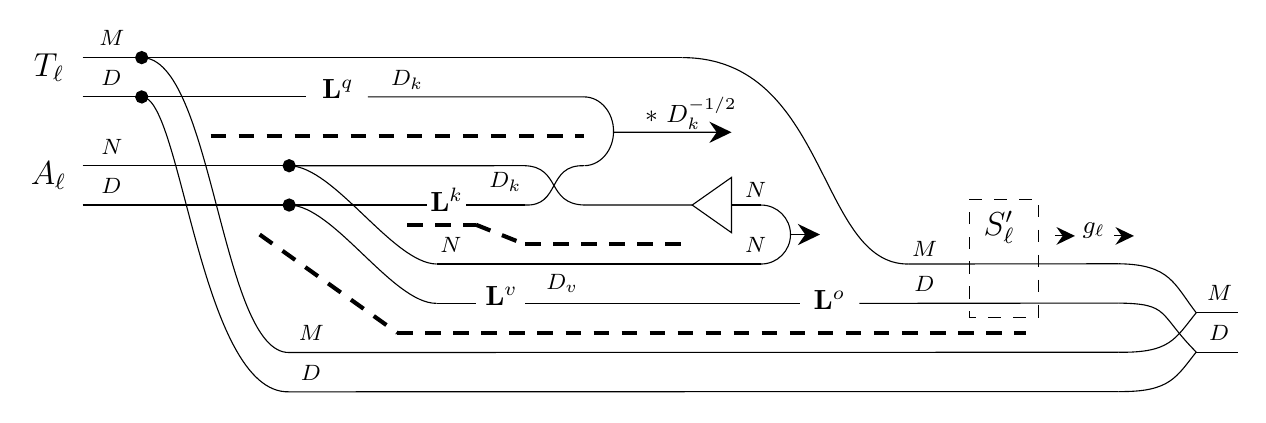
\begin{tikzpicture}[x=0.75pt,y=0.75pt,yscale=-1,xscale=1]
%uncomment if require: \path (0,209); %set diagram left start at 0, and has height of 209

%Straight Lines [id:da9318541924872752] 
\draw [color={rgb, 255:red, 0; green, 0; blue, 0 }  ,draw opacity=1 ]   (28.52,24.09) -- (317.42,24.09) ;
%Straight Lines [id:da9479457685518922] 
\draw [color={rgb, 255:red, 0; green, 0; blue, 0 }  ,draw opacity=1 ]   (284.27,60.08) -- (338.1,60.07) ;
\draw [shift={(341.1,60.07)}, rotate = 179.99] [fill={rgb, 255:red, 0; green, 0; blue, 0 }  ,fill opacity=1 ][line width=0.08]  [draw opacity=0] (10.72,-5.15) -- (0,0) -- (10.72,5.15) -- (7.12,0) -- cycle    ;
%Straight Lines [id:da9416679881824883] 
\draw [color={rgb, 255:red, 0; green, 0; blue, 0 }  ,draw opacity=1 ]   (28.52,43.04) -- (136.25,43.04) ;
%Straight Lines [id:da820033648196937] 
\draw [color={rgb, 255:red, 0; green, 0; blue, 0 }  ,draw opacity=1 ]   (28.52,76.19) -- (127.98,76.19) ;
%Straight Lines [id:da3464705312194676] 
\draw [color={rgb, 255:red, 0; green, 0; blue, 0 }  ,draw opacity=1 ]   (28.52,95.13) -- (127.98,95.13) ;
%Straight Lines [id:da6907623082124388] 
\draw [color={rgb, 255:red, 0; green, 0; blue, 0 }  ,draw opacity=1 ][line width=1.5]  [dash pattern={on 5.63pt off 4.5pt}]  (90.09,61.98) -- (270.06,61.98) ;
%Straight Lines [id:da2178356496804179] 
\draw [color={rgb, 255:red, 0; green, 0; blue, 0 }  ,draw opacity=1 ]   (199.02,123.55) -- (355.31,123.55) ;
%Shape: Arc [id:dp9189314153891996] 
\draw  [draw opacity=0] (270.28,76.17) .. controls (278.02,76.03) and (284.27,68.67) .. (284.27,59.6) .. controls (284.27,50.44) and (277.91,43.02) .. (270.06,43.02) .. controls (270.04,43.02) and (270.01,43.02) .. (269.99,43.02) -- (270.06,59.6) -- cycle ; \draw  [color={rgb, 255:red, 0; green, 0; blue, 0 }  ,draw opacity=1 ] (270.28,76.17) .. controls (278.02,76.03) and (284.27,68.67) .. (284.27,59.6) .. controls (284.27,50.44) and (277.91,43.02) .. (270.06,43.02) .. controls (270.04,43.02) and (270.01,43.02) .. (269.99,43.02) ;  
%Curve Lines [id:da9542147110842154] 
\draw [color={rgb, 255:red, 0; green, 0; blue, 0 }  ,draw opacity=1 ]   (241.64,76.17) .. controls (258.95,76.9) and (252,94.58) .. (270.06,95.12) ;
%Curve Lines [id:da811837651150005] 
\draw [color={rgb, 255:red, 0; green, 0; blue, 0 }  ,draw opacity=1 ]   (241.64,95.12) .. controls (258.95,95.84) and (252,75.63) .. (270.06,76.17) ;
%Straight Lines [id:da9225972703365359] 
\draw [color={rgb, 255:red, 0; green, 0; blue, 0 }  ,draw opacity=1 ]   (270.06,95.12) -- (322.16,95.13) ;
%Shape: Arc [id:dp012632027617723418] 
\draw  [draw opacity=0] (355.31,123.55) .. controls (363.16,123.55) and (369.52,117.19) .. (369.52,109.34) .. controls (369.52,101.5) and (363.16,95.13) .. (355.31,95.13) -- (355.31,109.34) -- cycle ; \draw  [color={rgb, 255:red, 0; green, 0; blue, 0 }  ,draw opacity=1 ] (355.31,123.55) .. controls (363.16,123.55) and (369.52,117.19) .. (369.52,109.34) .. controls (369.52,101.5) and (363.16,95.13) .. (355.31,95.13) ;  
%Straight Lines [id:da8996757312086063] 
\draw [color={rgb, 255:red, 0; green, 0; blue, 0 }  ,draw opacity=1 ]   (341.1,95.13) -- (355.31,95.13) ;
%Shape: Triangle [id:dp9355169581622589] 
\draw   (322.16,95.13) -- (341.1,81.81) -- (341.1,108.45) -- cycle ;
%Straight Lines [id:da9948364456698844] 
\draw [color={rgb, 255:red, 0; green, 0; blue, 0 }  ,draw opacity=1 ]   (369.52,109.34) -- (380.73,109.34) ;
\draw [shift={(383.73,109.34)}, rotate = 180] [fill={rgb, 255:red, 0; green, 0; blue, 0 }  ,fill opacity=1 ][line width=0.08]  [draw opacity=0] (10.72,-5.15) -- (0,0) -- (10.72,5.15) -- (7.12,0) -- cycle    ;
%Straight Lines [id:da6043160547682214] 
\draw [color={rgb, 255:red, 0; green, 0; blue, 0 }  ,draw opacity=1 ]   (426.35,123.55) -- (527.64,123.42) ;
%Curve Lines [id:da6867804311377057] 
\draw [color={rgb, 255:red, 0; green, 0; blue, 0 }  ,draw opacity=1 ]   (317.42,24.09) .. controls (387.99,24.27) and (382.54,123.97) .. (426.35,123.55) ;
%Curve Lines [id:da35185424855257263] 
\draw [color={rgb, 255:red, 0; green, 0; blue, 0 }  ,draw opacity=1 ]   (127.98,76.19) .. controls (149.75,76.35) and (177.86,123.17) .. (199.02,123.55) ;
\draw [shift={(127.98,76.19)}, rotate = 0.42] [color={rgb, 255:red, 0; green, 0; blue, 0 }  ,draw opacity=1 ][fill={rgb, 255:red, 0; green, 0; blue, 0 }  ,fill opacity=1 ][line width=0.75]      (0, 0) circle [x radius= 2.68, y radius= 2.68]   ;
%Straight Lines [id:da1325813172340935] 
\draw [color={rgb, 255:red, 0; green, 0; blue, 0 }  ,draw opacity=1 ][line width=1.5]  [dash pattern={on 5.63pt off 4.5pt}]  (241.64,114.08) -- (322.16,114.08) ;
%Curve Lines [id:da1474512418867049] 
\draw [color={rgb, 255:red, 0; green, 0; blue, 0 }  ,draw opacity=1 ]   (127.98,95.13) .. controls (149.51,95.3) and (177.86,142.66) .. (199.02,142.5) ;
\draw [shift={(127.98,95.13)}, rotate = 0.43] [color={rgb, 255:red, 0; green, 0; blue, 0 }  ,draw opacity=1 ][fill={rgb, 255:red, 0; green, 0; blue, 0 }  ,fill opacity=1 ][line width=0.75]      (0, 0) circle [x radius= 2.68, y radius= 2.68]   ;
%Straight Lines [id:da0024795885398030126] 
\draw [color={rgb, 255:red, 0; green, 0; blue, 0 }  ,draw opacity=1 ]   (165.87,43.04) -- (269.99,43.02) ;
%Straight Lines [id:da5129391997953758] 
\draw [color={rgb, 255:red, 0; green, 0; blue, 0 }  ,draw opacity=1 ]   (213.23,95.13) -- (241.64,95.13) ;
%Straight Lines [id:da5222565283453322] 
\draw [color={rgb, 255:red, 0; green, 0; blue, 0 }  ,draw opacity=1 ]   (199.02,142.5) -- (217.96,142.5) ;
%Straight Lines [id:da5713516733511401] 
\draw [color={rgb, 255:red, 0; green, 0; blue, 0 }  ,draw opacity=1 ]   (241.64,142.5) -- (374.25,142.5) ;
%Straight Lines [id:da7381871923413768] 
\draw [color={rgb, 255:red, 0; green, 0; blue, 0 }  ,draw opacity=1 ][line width=1.5]  [dash pattern={on 5.63pt off 4.5pt}]  (184.81,104.61) -- (217.96,104.61) ;
%Straight Lines [id:da4800244787455168] 
\draw [color={rgb, 255:red, 0; green, 0; blue, 0 }  ,draw opacity=1 ][line width=1.5]  [dash pattern={on 5.63pt off 4.5pt}]  (217.96,104.61) -- (241.64,114.08) ;
%Straight Lines [id:da3222725473972332] 
\draw [color={rgb, 255:red, 0; green, 0; blue, 0 }  ,draw opacity=1 ]   (402.67,142.5) -- (527.64,142.37) ;
%Shape: Rectangle [id:dp5331533235436763] 
\draw  [dash pattern={on 4.5pt off 4.5pt}] (455.71,92.29) -- (488.87,92.29) -- (488.87,149.13) -- (455.71,149.13) -- cycle ;
%Curve Lines [id:da5832391229104559] 
\draw [color={rgb, 255:red, 0; green, 0; blue, 0 }  ,draw opacity=1 ]   (56.94,43.04) .. controls (76.07,42.2) and (85.17,186.36) .. (127.98,185.12) ;
\draw [shift={(56.94,43.04)}, rotate = 357.48] [color={rgb, 255:red, 0; green, 0; blue, 0 }  ,draw opacity=1 ][fill={rgb, 255:red, 0; green, 0; blue, 0 }  ,fill opacity=1 ][line width=0.75]      (0, 0) circle [x radius= 2.68, y radius= 2.68]   ;
%Curve Lines [id:da07594588484193321] 
\draw [color={rgb, 255:red, 0; green, 0; blue, 0 }  ,draw opacity=1 ]   (56.94,24.09) .. controls (91.23,24.01) and (95.02,166.66) .. (127.98,166.18) ;
\draw [shift={(56.94,24.09)}, rotate = 359.86] [color={rgb, 255:red, 0; green, 0; blue, 0 }  ,draw opacity=1 ][fill={rgb, 255:red, 0; green, 0; blue, 0 }  ,fill opacity=1 ][line width=0.75]      (0, 0) circle [x radius= 2.68, y radius= 2.68]   ;
%Straight Lines [id:da4069702799953998] 
\draw [color={rgb, 255:red, 0; green, 0; blue, 0 }  ,draw opacity=1 ]   (127.98,166.18) -- (527.64,166.05) ;
%Straight Lines [id:da04501569766126101] 
\draw [color={rgb, 255:red, 0; green, 0; blue, 0 }  ,draw opacity=1 ]   (127.98,185.12) -- (527.64,184.99) ;
%Straight Lines [id:da10656219889721918] 
\draw [color={rgb, 255:red, 0; green, 0; blue, 0 }  ,draw opacity=1 ]   (525.53,110) -- (532,110) ;
\draw [shift={(535,110)}, rotate = 180] [fill={rgb, 255:red, 0; green, 0; blue, 0 }  ,fill opacity=1 ][line width=0.08]  [draw opacity=0] (8.93,-4.29) -- (0,0) -- (8.93,4.29) -- (5.93,0) -- cycle    ;
%Straight Lines [id:da8097902856805503] 
\draw [color={rgb, 255:red, 0; green, 0; blue, 0 }  ,draw opacity=1 ]   (497.11,110) -- (503.58,110) ;
\draw [shift={(506.58,110)}, rotate = 180] [fill={rgb, 255:red, 0; green, 0; blue, 0 }  ,fill opacity=1 ][line width=0.08]  [draw opacity=0] (8.93,-4.29) -- (0,0) -- (8.93,4.29) -- (5.93,0) -- cycle    ;
%Curve Lines [id:da8240921966457793] 
\draw [color={rgb, 255:red, 0; green, 0; blue, 0 }  ,draw opacity=1 ]   (527.64,123.42) .. controls (552.56,123.76) and (554.33,133.2) .. (565,147.02) ;
%Curve Lines [id:da8752997693066615] 
\draw [color={rgb, 255:red, 0; green, 0; blue, 0 }  ,draw opacity=1 ]   (527.64,166.05) .. controls (552.56,166.38) and (554.78,159.65) .. (565,147.02) ;
%Curve Lines [id:da10181116987059924] 
\draw [color={rgb, 255:red, 0; green, 0; blue, 0 }  ,draw opacity=1 ]   (527.64,142.37) .. controls (552.56,142.7) and (546.42,147.31) .. (565,165.97) ;
%Curve Lines [id:da853323633730164] 
\draw [color={rgb, 255:red, 0; green, 0; blue, 0 }  ,draw opacity=1 ]   (527.64,184.99) .. controls (552.56,185.32) and (555.44,177.87) .. (565,165.97) ;
%Straight Lines [id:da546971982487424] 
\draw    (565,147.02) -- (585,147.02) ;
%Straight Lines [id:da31488236797131886] 
\draw    (565,165.97) -- (585,165.97) ;
%Straight Lines [id:da615457324230881] 
\draw [color={rgb, 255:red, 0; green, 0; blue, 0 }  ,draw opacity=1 ][line width=1.5]  [dash pattern={on 5.63pt off 4.5pt}]  (180.08,156.7) -- (483.18,156.7) ;
%Straight Lines [id:da1734793752436845] 
\draw [color={rgb, 255:red, 0; green, 0; blue, 0 }  ,draw opacity=1 ]   (127.98,95.13) -- (194.28,95.13) ;
%Straight Lines [id:da411491139550342] 
\draw [color={rgb, 255:red, 0; green, 0; blue, 0 }  ,draw opacity=1 ]   (127.98,76.19) -- (241.64,76.17) ;
%Straight Lines [id:da36908543265196636] 
\draw [color={rgb, 255:red, 0; green, 0; blue, 0 }  ,draw opacity=1 ][line width=1.5]  [dash pattern={on 5.63pt off 4.5pt}]  (113.77,109.34) -- (180.08,156.7) ;

% Text Node
\draw (35.23,9.94) node [anchor=north west][inner sep=0.75pt]  [font=\fontsize{0.82em}{0.99em}\selectfont]  {$M$};
% Text Node
\draw (3.76,21.05) node [anchor=north west][inner sep=0.75pt]  [font=\large]  {$T_{\ell }$};
% Text Node
\draw (36.23,28.89) node [anchor=north west][inner sep=0.75pt]  [font=\fontsize{0.82em}{0.99em}\selectfont]  {$D$};
% Text Node
\draw (2.26,73.14) node [anchor=north west][inner sep=0.75pt]  [font=\large]  {$A_{\ell }$};
% Text Node
\draw (36.23,80.98) node [anchor=north west][inner sep=0.75pt]  [font=\fontsize{0.82em}{0.99em}\selectfont]  {$D$};
% Text Node
\draw (36.23,62.04) node [anchor=north west][inner sep=0.75pt]  [font=\fontsize{0.82em}{0.99em}\selectfont]  {$N$};
% Text Node
\draw (298.21,41.97) node [anchor=north west][inner sep=0.75pt]  [font=\small]  {$*\ D_{k}^{-1/2}$};
% Text Node
\draw (142.61,33.5) node [anchor=north west][inner sep=0.75pt]  [font=\normalsize]  {$\mathbf{L}^{q}$};
% Text Node
\draw (175.79,28.86) node [anchor=north west][inner sep=0.75pt]  [font=\fontsize{0.82em}{0.99em}\selectfont]  {$D_{k}$};
% Text Node
\draw (194.7,85.59) node [anchor=north west][inner sep=0.75pt]  [font=\normalsize]  {$\mathbf{L}^{k}$};
% Text Node
\draw (223.15,78.12) node [anchor=north west][inner sep=0.75pt]  [font=\fontsize{0.82em}{0.99em}\selectfont]  {$D_{k}$};
% Text Node
\draw (221.22,132.95) node [anchor=north west][inner sep=0.75pt]  [font=\normalsize]  {$\mathbf{L}^{v}$};
% Text Node
\draw (250.61,127.37) node [anchor=north west][inner sep=0.75pt]  [font=\fontsize{0.82em}{0.99em}\selectfont]  {$D_{v}$};
% Text Node
\draw (199.62,109.4) node [anchor=north west][inner sep=0.75pt]  [font=\fontsize{0.82em}{0.99em}\selectfont]  {$N$};
% Text Node
\draw (346.44,82.88) node [anchor=north west][inner sep=0.75pt]  [font=\fontsize{0.82em}{0.99em}\selectfont]  {$N$};
% Text Node
\draw (346.44,109.4) node [anchor=north west][inner sep=0.75pt]  [font=\fontsize{0.82em}{0.99em}\selectfont]  {$N$};
% Text Node
\draw (461.29,96.82) node [anchor=north west][inner sep=0.75pt]  [font=\large]  {$S'_{\ell }$};
% Text Node
\draw (379.41,134.85) node [anchor=north west][inner sep=0.75pt]  [font=\normalsize]  {$\mathbf{L}^{o}$};
% Text Node
\draw (426.9,111.29) node [anchor=north west][inner sep=0.75pt]  [font=\fontsize{0.82em}{0.99em}\selectfont]  {$M$};
% Text Node
\draw (427.9,128.34) node [anchor=north west][inner sep=0.75pt]  [font=\fontsize{0.82em}{0.99em}\selectfont]  {$D$};
% Text Node
\draw (509,102.4) node [anchor=north west][inner sep=0.75pt]  [font=\small]  {$g_{\ell }$};
% Text Node
\draw (569,132.4) node [anchor=north west][inner sep=0.75pt]  [font=\fontsize{0.82em}{0.99em}\selectfont]  {$M$};
% Text Node
\draw (570,151.82) node [anchor=north west][inner sep=0.75pt]  [font=\fontsize{0.82em}{0.99em}\selectfont]  {$D$};
% Text Node
\draw (131.37,152.02) node [anchor=north west][inner sep=0.75pt]  [font=\fontsize{0.82em}{0.99em}\selectfont]  {$M$};
% Text Node
\draw (132.37,170.97) node [anchor=north west][inner sep=0.75pt]  [font=\fontsize{0.82em}{0.99em}\selectfont]  {$D$};
\end{tikzpicture}
}
\sidecaption{Neural circuit diagram for the proposed SAM-Decoder-Adapter following the methodology described in~\cite{abbott2024neural}.\label{fig:neural_diagram}
}
\end{figure}

We note that this approach could potentially be implemented within the model's encoder. However, we deliberately decided not to pursue this route for two main reasons: (1) the image representation generated by the encoder is already high-quality due to a pre-trained model on similar data, and (2) any modifications to the encoder's parameters may necessitate retraining of the mask decoder as well. Given our objective of reducing the number of parameters, we confine the implementation solely to the decoder. In \Cref{sec:ablation_samda}, we show experimentally how the location of the adapter affects the model's performance.

\section{Experimental setup}
\label{sec:experiments}
%% Points:
%% - Datasets: Retouch, MRI (Binary), ...
%% - Hyperparameters are tuned for each experiment on the validation set, then applied to testing. Probably a table with the hyperparams doesn't fit
%% - Baselines
%% - Supervised training, TTDA
The following section details our experimental setup and compares our approach to several baselines. We apply our method to two scenarios: fully-supervised semantic segmentation and test-time domain adaptation (TTDA) for semantic segmentation on four datasets.

\subsection{Datasets}
We validate our approach on one natural image dataset and three medical cross-device/site datasets:
\begin{itemize}
    \item{\textbf{Retouch}\sideauthorcite{retouch}}: Retinal OCT volumes from three devices - Cirrus, Spectralis, and Topcon devices - including segmentation masks for three biological markers: IRF, SRF, and PED. We use ``Spectralis'' dataset as the source and ``Cirrus'' dataset as the target domain. 
    
    % Retinal OCT volumes acquired with three different devices: Cirrus HD-OCT (Zeiss, Meditec), Spectralis (Heidelberg Engineering), and T-1000/T2000 (Topcon). The volumes contain segmentation masks for three retinal biological markers: IRF, SRF, and PED. For TTDA, we use ``Spectralis'' dataset as the source and ``Cirrus'' dataset as the target domain.
    
    \item{\textbf{MRI}\sideauthorcite{liu2020saml,liu2020ms}}: Prostate MRI scans from various sites with different devices showing prostate capsule segmentation at various cancer stages. We extract subsets from Boston Medical Center (BMC) and University College London (UCL). ``BMC'' serves as the source domain, while ``UCL'' is the target.
    
    %Prostate T2-weighted MRI acquired at multiple sites with different devices. Each MRI contains a segmentation of the prostate capsule at different stages of cancer. We extract two subsets from different sites: Boston Medical Center (BMC) and University College London (UCL). For TTDA, we sample volumes from ``BMC'' and ``UCL'' as the source and target domain, respectively. 
    
    \item{\textbf{WMH}\sideauthorcite{wmh}}: Brain MRI scans from three sites: NUHS Singapore, UMC Utrecht, and VU Amsterdam, with White Matter Hyperintensities and other pathologies segmented. We extract FLAIR axial slices containing segmentation. We take ``UMC Utrecht'' as the source, and ``NUHS Singapore'' as the target domain.
    
    % Brain T1-weighted and FLAIR MRI acquired at three sites with different devices: National University Health System in Singapore (NUHS Singapore), University Medical Center Utrecht (UMC Utrecht), and VU University Medical Centre Amsterdam (VU Amsterdam). Each MRI contains a segmentation of WMH and other pathologies (grouped). We extract all axial slices from the FLAIR MRI containing segmentation. For TTDA, we sample volumes from ``UMC Utrecht'' and ``NUHS Singapore'' as the source and target domain, respectively. 

    \item{\textbf{HQSeg-44K}\sideauthorcite{ke2024segment}} contains a collection of datasets for training and testing. For training, data is taken from DIS\sidecite{qin2022highly} (train set), ThinObject-5K\sidecite{coift_liew2021deep} (train set), FSS-1000\sidecite{fss_li2020fss}, ECSSD\sidecite{eccsd_shi2015hierarchical}, MSRA10K\sidecite{msra_cheng2014global} and DUT-OMRON\sidecite{dutomron_yang2013saliency}. The models are tested on a collection of four datasets: DIS (validation set), ThinObject-5K (test set), COIFT\sidecite{coift_liew2021deep}, and HRSOD\sidecite{hrsod_zeng2019towards}. These datasets contain fine-grained mask labels of natural images and together they add up to more than 1,000 semantic classes. 
    
\end{itemize}
In all cases, we use the source domain as the only domain for the fully supervised experiments. Since HQSeg-44K contains natural images with no clear domain shift, we do not report results for generalization and domain adaptation on this dataset. We report all the results on separate test sets, following hyperparameter fine-tuning on a validation set and repeating each experiment four times. \Cref{tab:dataset_details_samda} describes the size of the training, validation, and test splits for each dataset and domain. 

\begin{table}[]
\centering
\sidecaption{Number of images for each dataset per split. HQSeg-44K is a combination of datasets~\parencite{ke2024segment} and it uses the same set for validation and testing.\label{tab:dataset_details_samda}}

\begin{tabular}{@{}p{2.5cm}lP{2cm}P{1.8cm}P{1.8cm}@{}}
\toprule
\multicolumn{1}{l}{{Dataset}} & {Domains} & {Training} & {Validation} & {Test} \\ \midrule
\multirow{2}{*}{Retouch} & Spectralis & 1,773 & 591 & 480 \\
 & Cirrus & 3,765 & 1,255 & 1,252 \\ \midrule
\multirow{2}{*}{MRI} & BMC & 177 & 92 & 93 \\
 & UCL & 82 & 41 & 41 \\ \midrule
\multirow{2}{*}{WMH} & Utrecht & 4,260 & 1,065 & 1,255 \\
 & Singapore & 3,560 & 890 & 1,105 \\ \midrule
HQSeg-44k & - & 44,320 & \multicolumn{2}{c}{1,537} \\
 
 \bottomrule
\end{tabular}

\end{table}

\subsection{Baselines}
We compare our adapter against four alternative techniques. Among these, three are prominent examples of contemporary state-of-the-art approaches: LoRA\sidecite{hu2022lora}, Med-SA\sidecite{wu2023medical} and HQ-SAM\sidecite{ke2024segment}. The remaining methods involve completely fine-tuning the model and solely fine-tuning the decoder while keeping the encoder frozen. It is important to acknowledge that certain methods alter the image embedding as they are integrated within the encoder. To ensure equitable comparisons, we train both the adapter and the mask decoder in these cases. We use the ViT-B/16\sidecite{dosovitskiy2021an} variant of the Vision Transformer pre-trained with MedSAM\sidecite{MedSAM} weights for all our experiments on medical datasets and the official SAM pre-training weights for HQSeg-44K.


\subsection{Fully Supervised Training Experiments}
Here, we evaluate SAM Decoder Adapter through fully supervised semantic segmentation training on individual images and evaluate the models on the same training domain and a different domain\sidenote{Unlike previous literature on SAM, we perform all of our experiments without prompting, and leave prompting adaption to further work.}. 
We use AdamW\sidecite{loshchilov2017decoupled} optimizer in all cases with a loss that combines a \emph{mask prediction loss} and a \emph{IoU prediction loss}. The mask prediction loss is a linear combination of Dice loss\sidecite{milletari2016dice} and Cross Entropy loss in a 0.8:0.2 ratio. The IoU prediction loss is used to train the IoU prediction head of SAM. It is computed as the MSE between the IoU prediction of SAM and the IoU of the predicted mask with the ground truth mask. As reported in~\yeartextcite{sam}, using this IoU prediction loss with a weight of 1.0 increases performance slightly. Other hyperparameters are fine-tuned with the validation set. Our adapter uses $N=2$~tokens and dimension~$D=512$. The dimensions of the attention module are~$D_v=D_k=256$.

\subsection{Test-Time Domain Adaptation Experiments}
Test-time domain adaptation (TTDA) refers to a scenario in which a model receives unlabeled data during inference from a dataset with a data distribution that differs from that on which it was trained. Accordingly, the model must adapt on a sample-by-sample basis, attempting to extract the maximum amount of information from each data point. In these experiments, we assume that the domain shift between the source and target distributions is due solely to differences in the acquisition device and, therefore, that the class semantics and number of classes remain unchanged. This scenario is not hypothetical in clinical practice: a model trained to detect biological markers with a specific configuration of the image acquisition device can be required to adapt to a new configuration, but the underlying detection scheme (number and semantics of classes) will remain the same.

\begin{margintable}[]\small
\caption{Number of trainable parameters for each method}
\label{tab:trainable_params}
\begin{tabular}{@{}lP{20mm}@{}}
\toprule
\textbf{Method}       & \textbf{Learnable  Params (M)}\\ \midrule
Fine-Tuning                         & 90.60     \\
Decoder FT                          & 3.92      \\
LoRA~\cite{hu2022lora}              & 4.07      \\
Med-SA~\cite{wu2023medical}         & 11.03     \\
HQ-SAM~\cite{ke2024segment}         & 1.07      \\
SAM-DA                              & 0.66      \\ \bottomrule
\end{tabular}
\end{margintable}

We adopt a conventional training approach centered on entropy minimization per sample, leveraging the most confident samples\sidecite{wang2021tent}. Then, we enforce proximity between the output and initial predictions through a regularization term incorporating focal loss\sidecite{lin2017focal} and dice loss, following \yeartextcite{zhang2023improving}. Finally, for Retouch we introduce a contrastive term within the volume. Negative slices are sampled distantly from the anchor, while positive slices are nearby. We optimize the contribution of each term to the final loss for every method and dataset on the validation set, as well as the number of iterations. We zero-initialize the adapter of the Med-SA baseline, ensuring that it does not affect the model predictions before adaptation. Due to the challenge of zero-initializing HQ-SAM, we omit it from these experiments.

Note that the adapter we propose in this paper is agnostic to the test-time domain adaptation algorithm. For this reason, we opt to use a simple training approach that will not shade the adapter's capabilities. Furthermore, comparisons are only carried out against other adapters and PEFT methods. Comparing against different test-time domain adaptation techniques would be out of the scope of the present work.
\section{Results}
\label{sec:samda_results}
%% Points:
%% - Supervised experiments (table 1) + zero-shot (table 2)
%% - TTDA experiments (table 3)
%% - Some images showing the evolution <-- Save ckpts for some imgs then

\plainwidefig[t]{1}{Figures/full_supervision_MICCAI.pdf}{Qualitative results on eight randomly selected test samples.}{fig:full_superv}

\subsection{Full Supervision}
\Cref{tab:supervised_training} presents a comparison of the IoU scores achieved by SAM Decoder Adapter (SAM-DA) against alternative baselines across four datasets in the fully supervised task. Our approach consistently delivers comparable or superior results to full fine-tuning despite employing only a fraction of the trainable parameters\sidenote{See \Cref{tab:trainable_params}}. Notably, the number of training images influences the model's final performance: the BMC domain in the MRI dataset, with the fewest samples across all datasets, showcases significant performance improvement with our adapter compared to other methods. With fewer parameters, SAM Decoder Adapter is less susceptible to overfit to the training set, thereby retaining valuable knowledge from the pre-trained weights. This effect diminishes as the dataset size increases, where the advantage of the adapter over competitive baselines is less evident. \cref{fig:full_superv} shows qualitative results of our adapter.

\begin{table}[t]
\sidecaption{IoU scores for the full supervision task. Variances are computed over four trained models on the validation set. Bold numbers indicate the best adapter. Asterisks indicate the second best. Learnable parameters refer to the number of parameters that are trained for each method.\label{tab:supervised_training}}
\centering
\begin{tabular}{@{}p{3cm}P{2cm}P{1.4cm}P{1.4cm}P{1.75cm}@{}}
\toprule
  & Retouch - Spectralis & MRI - BMC & WMH - Utrecht & HQSeg-44K  \\ \midrule
Fine-Tuning &  $76.0{\scriptstyle \pm 0.6}$ & $85.9{\scriptstyle \pm 1.5}$ & $43.5{\scriptstyle \pm 0.9}$ & $76.0{\scriptstyle \pm 0.3}$  \\ \midrule
Decoder FT  & $42.8{\scriptstyle \pm 2.0}$ & $71.9{\scriptstyle \pm 2.6}$ & $40.8{\scriptstyle \pm 0.3}$ & $80.9{\scriptstyle \pm 0.3}$  \\
LoRA~{\footnotesize\parencite{hu2022lora}} & $74.1{\scriptstyle \pm 1.1}$ & $83.7{\scriptstyle \pm 1.3}$ & $43.1{\scriptstyle \pm 0.5}$ & $83.1{\scriptstyle \pm 0.3}$*  \\
Med-SA~{\footnotesize\parencite{wu2023medical}}  & $75.0{\scriptstyle \pm 1.2}$* & $84.3{\scriptstyle \pm 1.9}$* & $\mathbf{44.7}{\scriptstyle \pm 0.7}$ & $\mathbf{83.8}{\scriptstyle \pm 0.4}$  \\
HQ-SAM~{\footnotesize\parencite{ke2024segment}}  & $52.4{\scriptstyle \pm 2.1}$ & $76.5{\scriptstyle \pm 1.5}$ & $40.9{\scriptstyle \pm 0.6}$ & $79.2{\scriptstyle \pm 0.2}$  \\ \midrule
SAM-DA  & $\mathbf{75.4}{\scriptstyle \pm 0.6}$ & $\mathbf{86.2}{\scriptstyle \pm 1.5}$ & $44.2{\scriptstyle \pm 0.3}$* & $79.6{\scriptstyle \pm 0.4}$  \\ \bottomrule
\end{tabular}
\end{table}

\begin{table}[htbp]
\sidecaption{Domain generalization results on an unseen domain (IoU score). Variances are computed over four trained models on the validation set.\label{tab:zero_shot}}
\centering
\begin{tabular}{@{}p{3cm}P{2.4cm}P{2cm}P{2.6cm}@{}}
\toprule
 & Retouch - Cirrus & MRI - UCL & WMH - Singapore \\ \midrule
Fine-Tuning & $65.4{\scriptstyle \pm 5.1}$ & $80.9{\scriptstyle \pm 1.1}$ & $40.1{\scriptstyle \pm 0.9}$ \\ \midrule
Decoder FT & $27.0{\scriptstyle \pm 0.7}$ & $70.4{\scriptstyle \pm 0.8}$ & $35.8{\scriptstyle \pm 0.95}$ \\
LoRA~{\footnotesize\parencite{hu2022lora}} & $56.0{\scriptstyle \pm 5.6}$ & $75.9{\scriptstyle \pm 1.5}$ & $37.3{\scriptstyle \pm 1.0}$ \\
Med-SA~{\footnotesize\parencite{wu2023medical}} & $61.7{\scriptstyle \pm 3.5}$ & $75.8{\scriptstyle \pm 7.0}$ & $38.8{\scriptstyle \pm 1.2}$ \\
HQ-SAM~{\footnotesize\parencite{ke2024segment}} & $30.8{\scriptstyle \pm 0.4}$ & $75.8{\scriptstyle \pm 3.7}$ & $35.9{\scriptstyle \pm 0.7}$ \\ \midrule
SAM-DA & $\mathbf{70.2}{\scriptstyle \pm 3.1}$ & $\mathbf{80.6}{\scriptstyle \pm 1.0}$ & $\mathbf{39.6}{\scriptstyle \pm 0.7}$ \\ \bottomrule
\end{tabular}
\end{table}



Due to the substantial number of images in HQSeg-44K\sideauthorcite{ke2024segment}, this dataset can be considered quite distinct. With 44k training images, encoder-adaptation methods are expected to outperform decoder-only approaches due to their higher number of parameters. Our method achieves an IoU score of 79.6 on this dataset, falling behind LoRA and Med-SA (with an average IoU of 83.5). However, it surpasses other decoder-only adapters like HQ-SAM, which achieves an IoU of 79.2. These results are the average over the four testing sets in HQSeg-44K, and the detailed figures can be found on \Cref{tab:hqseg_results_samda}.

\subsection{Domain Generalization}
One of the primary strengths of SAM lies in its ability to zero-shot transfer thanks to its extensive pre-training corpus. We investigate in \Cref{tab:zero_shot} whether this capability is retained after the adaption by testing the methods from \Cref{tab:supervised_training} on previously unseen domains within each medical dataset. SAM Decoder Adapter demonstrates statistically significant superiority in zero-shot generalization compared to other methods that primarily focus on traditional encoder adaptation, such as Med-SA and LoRA, and shows on-par performance to fine-tuning in the low-data regime. See supplementary material for qualitative results of our adapter compared to two baselines on the generalization domains.

\subsection{Ablation study}\label{sec:ablation_samda}
The Vision Transformer-type architecture used in the backbone of SAM facilitates the seamless integration of the proposed adapter into the encoder with minimal adjustments compared to the configuration depicted in \cref{fig:method_samda}. We adopt the approach outlined in \yeartextcite{llama_adapter} to position the adapter within the encoder, focusing on adapting only the last layers. Additionally, we utilize all image embeddings as queries for the attention module and fine-tune the decoder, following the setting from LoRA and Med-SA. ViT-B comprises 12 blocks, and we modify the last ten blocks in our adaptation approach. This adaptation strategy allocates $17.7$M trainable parameters to the encoder adaptation, in addition to $3.9$M parameters in the decoder. \Cref{tab:encoder_ablation_trained,tab:encoder_ablation_generalization} illustrate the impact of adapting the encoder layers compared to the proposed method. The results confirm that locating the adapter in the decoder improves generalization on unseen domains\sidenote{As seen in \Cref{tab:encoder_ablation_generalization}.}, especially in the case of Retouch and WMH datasets, where we see a gain of $8.5\%$ and $13.8\%$ in IoU score, respectively.

\begin{table}[]
\sidecaption{Ablation study evaluating two adapter locations. IoU scores for full supervision. Variances are obtained over four trained models on the validation set.\label{tab:encoder_ablation_trained}}
\centering
\begin{tabular}{@{}lP{2.1cm}P{2cm}P{2.1cm}P{2cm}@{}}
\toprule
 & Retouch - Spectralis & MRI - BMC & WMH - Utrecht & HQSeg-44K  \\ \midrule
Decoder & $75.4{\scriptstyle \pm 0.6}$ & $\mathbf{86.2}{\scriptstyle \pm 1.5}$ & $\mathbf{44.2}{\scriptstyle \pm 0.3}$ & $79.6{\scriptstyle \pm 0.4}$ \\
Encoder & $\mathbf{75.8}{\scriptstyle \pm 1.0}$ & $84.6{\scriptstyle \pm 2.2}$ & $40.7{\scriptstyle \pm 0.3}$ & $\mathbf{80.8}{\scriptstyle \pm 0.3}$ \\ \bottomrule 
\end{tabular}
\end{table}

\begin{table}[]
\sidecaption{Ablation study evaluating two adapter locations. IoU scores for domain generalization. Variances are obtained over four trained models on the validation set.\label{tab:encoder_ablation_generalization}}
\centering
\begin{tabular}{@{}lP{3cm}P{2.75cm}P{3cm}@{}}
\toprule
 & Retouch - Cirrus & MRI - UCL & WMH - Singapore  \\ \midrule
Decoder & $\mathbf{70.2}{\scriptstyle \pm 3.1}$ & $\mathbf{80.6}{\scriptstyle \pm 1.0}$ & $\mathbf{39.6}{\scriptstyle \pm 0.7}$ \\
Encoder & $64.7{\scriptstyle \pm 6.8}$ & $80.4{\scriptstyle \pm 1.4}$ & $34.8{\scriptstyle \pm 0.6}$ \\ \bottomrule
\end{tabular}
\end{table}

\Cref{tab:ablation_size,tab:ablation_size_transfer} in the appendix show the impact of the dimension of the adaptation prompt $A_\ell$ on the performance. The results do not suggest that the size of the adaptation prompt impacts the full supervision or the zero-shot generalization performance for the medical datasets significantly. For HQSeg-44K, however, the drop in performance when the size is increased is blatant. This is in line with the previous observation that decoder-only methods cannot trace encoder-decoder approaches in large datasets, and further adding parameters only promotes overfitting to the training set.

\subsection{Test-Time Domain Adaptation}
Due to the low number of trainable parameters, test-time domain adaptation is the ideal setting to test how much an adapter can affect the performance of a single test sample. We show in \Cref{tab:ttda} that our adapter performs better than other baselines in most cases. For MRI, the increase in trainable parameters already in LoRA hurts the initial model and decreases its IoU score after only five iterations. Our method, however, shows strong results in all three cases, as shown in \Cref{fig:ttda_samda} in the appendix.

\begin{table}
\sidecaption{Test-time domain adaptation results (IoU score). Due to the challenge of zero-initializing HQ-SAM, we omit it from these experiments.\label{tab:ttda}}
\centering
\begin{tabular}{@{}p{3cm}P{2.4cm}P{2cm}P{2.6cm}@{}}
\toprule
 & Retouch - Cirrus & MRI - UCL & WMH - Singapore \\ \midrule
Fine-Tuning & $61.2$ & $80.2$ & $39.6$ \\
Decoder FT & $66.9$ & $80.8$ & $40.4$ \\
LoRA~{\footnotesize\parencite{hu2022lora}} & $67.0$ & $80.7$ & $40.3$ \\
Med-SA~{\footnotesize\parencite{wu2023medical}} & $63.3$ & $80.7$ & $40.4$ \\ \midrule
%HQ-SAM~\parencite{ke2024segment} & - & - & - \\ \midrule
SAM-DA & $\mathbf{67.5}$ & $\mathbf{81.1}$ & $\mathbf{40.4}$ \\ \bottomrule
\end{tabular}
\end{table}

\section{Conclusion}
\label{sec:conclusion}
In this work, we propose a SAM Decoder Adapter for semantic segmentation that introduces negligible overhead. We achieve this by using a lean approach, using the image embeddings in the decoder as queries in the attention modules of the adapter, and combining the result before the next two-way attention layer. We outperform the mask prediction quality of state-of-the-art methods and show that zero-shot generalization capabilities are improved. Furthermore, we evaluate our method on a more challenging task, Test-Time Domain Adaptation, and show its superiority against other large model adapters. With extensive ablation studies, we explain the design choices behind this simple yet powerful adapter.
